\ProvidesFile{proofs.tex}[Доказательства]
\newpage
\section{Доказательства}
\subsection{Теорема Коши-Римана}
\begin{theorem}
  $f\in U(z_0)\to\C$, $f$ $\C$-дифференцируема в т. $z_0$ $\lra$ $f$ $\R$-дифференцируема и выполнено условие Коши-Римана:
  \[ 
  \begin{cases}
    u'_x = v'_y, \\
    u'_y=-v'_x, 
  \end{cases}\lra \p{f}{\overline{z}}(z_0)=0\]
\end{theorem}
\begin{proof}
 \begin{enumerate}
   \item[($\Rightarrow$):] $\Delta f = (a+ib)\Delta z + \overline{o}(\Delta z) = (a+ib)\Delta x + (ia-b)\Delta y + \overline{o}(\Delta z) = a\de x - b\de y + i(b\de x+ a\de y) +\overline{o}(\Delta z)=$
   \[=\begin{pmatrix}a&-b\\b&a\end{pmatrix}\begin{pmatrix}\de x\\\de y\end{pmatrix}+\overline{o}(\Delta z)\implies \p{f}{\overline{z}}(z_0) = \frac{a + ib -ib -a}{2} = 0\]
     \item[($\Leftarrow$):] При $\p{f}{\overline{z}}(z_0)=0$ уже показали, что $\de f = \p{f}{z}(z_0)\de z + 0 \cdot \overline{\de z} + \overline{o}(\de z)\implies f'(z_0) = \p{f}{z}(z_0)$
 \end{enumerate} 
\end{proof}
\subsection{Теорема о сохранение углов между кривыми под действием конформного\\ отображения}
\begin{theorem}
  Отображение $f$ конформно в $z_0$ и голоморфно в $\gamma_1,\gamma_2$. $\gamma_1,\gamma_2$ - гладкие кривые $\colon\q z_0\in \gamma_1,\gamma_2$. Тогда $\widetilde{\gamma_1}:=f(\gamma_1),\q \widetilde{\gamma_2}:=f(\gamma_2)$ - гладкие кривые, причём $\angle(\gamma_1,\gamma_2)|_{z_0} = \angle(\widetilde{\gamma_1},\widetilde{\gamma_2})|_{z_0}$ 
\end{theorem}
\begin{proof}
  Пусть $\g_i$ - параметризации $\gamma_i$. Тогда $f(\g_i)$ - параметризации $\widetilde{\gamma_i}$. $f(\g_i)\in C^1([0,1])$ по теореме о дифференцировании композиции, значит $\widetilde{\gamma_1},\q \widetilde{\gamma_2}$ - гладкие кривые. Рассмотрим производную: 
  \[(f(\g(t)))' = \begin{pmatrix}u'_x&u'_y\\v'_x&v'_y\end{pmatrix}\begin{pmatrix}x'(t)\\y'(t)\end{pmatrix}\]
    где $\begin{pmatrix}x'(t)\\y'(t)\end{pmatrix}\neq 0$, т.к. $\g_i$ гладкие, и $\begin{pmatrix}u'_x&u'_y\\v'_x&v'_y\end{pmatrix} = \begin{pmatrix}a&-b\\b&a\end{pmatrix}$, т.к. $f$ конформна. 
        \[0\neq |f'(z_0)| = \sqrt{a^2+b^2}\implies \det \begin{pmatrix}a&-b\\b&a\end{pmatrix}=a^2+b^2\neq 0\implies \text{ нет решений }\]
    т.е. угол не занулится. Вынесем $\sqrt{a^2+b^2}$ из матрицы и получим:
    \[(f(\g(t)))'=\sqrt{a^2+b^2}\begin{pmatrix}\cos\ph&-\sin\ph\\\sin\ph&\cos\ph\end{pmatrix}\begin{pmatrix}x'(t)\\y'(t)\end{pmatrix} \]
      Растяжение и поворот $\implies$ углы сохраняются, т.к. $\g_i'(t)=\begin{pmatrix}x_i'(t)\\y_i'(t)\end{pmatrix}$.
\end{proof}
\subsection{Круговое свойство ДЛО}
\begin{theorem}
  ДЛО переводит обобщённую окружность в обобщённую окружность.
\end{theorem}
\begin{proof}
    Для сдвига и поворота очевидно. Растяжение с центром в 0 очевидно, а растяжение не в 0: сдвиг в 0, растяжение, сдвиг обратно, т.е. $|a|z = |a|(z-z_0)+z_0|a|$

    Докажем, что уравнение обобщённой окружности имеет вид:
    \[Az\overline{z} + Bz+\overline{B}\overline{z}+C=0,\q A,C\in\R\]
    \begin{enumerate}
      \item $|z-z_0|^2=R^2$
      \[(z-z_0)(\overline{z}-\overline{z_0})=R^2\]
      \[z\overline{z} - \overline{z_0}z - z_0\overline{z} + z_0\overline{z_0} - R^2 = 0\]
      \[z\overline{z} - \overline{z_0}z - z_0\overline{z} + \left(|z_0|^2 - R^2\right) = 0\]
      \item $Ax+By+C=0$, где $x=\frac{z+\overline{z}}{2},\q y=\frac{z-\overline{z}}{2i}$
      \[A\frac{z+\overline{z}}{2} + B\frac{z-\overline{z}}{2i}+C=0\]
      \[0z\overline{z}+\left(\frac{A}{2} + \frac{B}{2i}\right)z + \left(\frac{A}{2} - \frac{B}{2i}\right)\overline{z} + C = 0\]
    \end{enumerate}
    Проверим теперь инверсию: $w=\frac{1}{z}\implies z = \frac{1}{w}$.
    \[Az\overline{z} + Bz+\overline{B}\overline{z}+C=0\]
    \[\frac{A}{w\overline{w}} + \frac{B}{w} + \frac{\overline{B}}{\overline{w}} + C = 0\q |\q \cdot w\overline{w}\]
    \[A + B\overline{w} + \overline{B}w + Cw\overline{w}=0\]
    Получили обобщённую окружность.
\end{proof}
\subsection{Правило трех точек для ДЛО}
\begin{theorem}
  $z_1,z_2,z_3\in\RC$ и $w_1,w_2,w_3\in\RC$. Тогда $\exists!\q w=f(z)$ - ДЛО : $w_k=f(z_k)$ 
\end{theorem}
\begin{proof}
   Доказательство только для случая $z_k\in\C,\q w_k\in\C$, т.к. лень.

  Рассмотрим отображение $f_1= 
  \begin{cases}
    z_1\mapsto 0\\
    z_2\mapsto \infty\\
    z_3\mapsto 1\\
  \end{cases}$, т.е.
  \[f_1=\frac{z-z_1}{z-z_2}\cdot \frac{z_3-z_2}{z_3-z_1}\]
  а также $f_2= 
  \begin{cases}
    w_1\mapsto 0\\
    w_2\mapsto \infty\\
    w_3\mapsto 1\\
  \end{cases}$, т.е.
  \[f_1=\frac{w-w_1}{w-w_2}\cdot \frac{w_3-w_2}{w_3-w_1}\]
  Значит искомое отображение $f=f_2^{-1}\circ f_1$. Покажем, что такое отображение единственно. Пусть $\exists \tilde{f}\colon z_k\mapsto w_k$. Тогда отображение
  \[F:=f_2\circ \tilde{f}\circ f_1^{-1} = 
  \begin{cases}
    0\mapsto 0\\
    \infty\mapsto \infty\\
    1\mapsto 1\\
  \end{cases}\]
  Заметим, что $\infty\mapsto \infty\lra F$ линейно, значит $F=Az+B$. $0\mapsto 0\lra B=0$. $1\mapsto 1\lra A=1$. Значит $F=z$, т.е.
  \[f_2\circ \tilde{f}\circ f_1^{-1}=id\lra \tilde{f} = f_2^{-1}\circ f_1=f\]
\end{proof}
\subsection{Лемма Гурса}
\begin{theorem}
  Пусть $f\in\O(D)$. Тогда $\forall \Delta\colon \overline{\de} \in D$ выполнено:
  \[\oint\limits_{\partial\de}f(z)\d z=0\]
\end{theorem}
\begin{proof}
  Пусть это неверно, т.е. $\exists \de \colon \overline{\de}\in D$ и 
  \[\oint\limits_{\partial\de}f(z)\d z = M>0\]

  Разобьём его на 4 $\de$ средними линиями.

  \begin{center}
  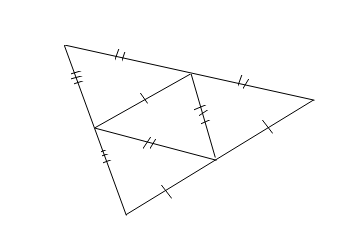
\includegraphics{2.png}
  \end{center}

  Обозначим $\de_1$ тот, где $\left|\oint\limits_{\partial\de}f(z)\d z\right|\geqslant \frac{M}{4}$. Продолжим цепочку разбиений. Получили $\overline{\de}\supset \overline{\de}_1\supset\dots\supset \overline{\de}_n\supset\dots$ - систему вложенных компактов. Значит $\exists z_0\colon z_0\in \bigcap_{n=0}^{\infty}\overline{\de}_n$, где $\overline{\de}_0:=\overline{\de}$ и
  \[\left|\oint\limits_{\partial\de_n}f(z)\d z\right|\geqslant \frac{M}{4^n}\]
  Так как диаметр $\de_n\to0$, то $\forall U(z_0)\q\exists N\in\N\colon \forall n>N\q \overline{\de}_n\subset U(z_0)$.

  По дано $f\in\O(z_0)$, значит $f$ $\C$-дифференцируема в $z_0$, т.е.
  \[f(z)=f(z_0) + f'(z_0)(z-z_0)+\al(z)(z-z_0)\]
  где $|\al(z)|<\e\q\forall z\in U_\delta(z_0)$. Тогда
  \[\oint\limits_{\partial\de_n}f(z)\d z = \oint\limits_{\partial\de_n}f(z_0)\d z + \oint\limits_{\partial\de_n}f'(z_0)(z-z_0)\d z + \oint\limits_{\partial\de_n}\al(z)(z-z_0)\d z\]
  Первые два интеграла в правой части равны 0, т.к., параметризовав их по определению, получим 0. Оценим оставшийся член:
  \[\left|\oint\limits_{\partial\de_n}\al(z)(z-z_0)\d z\right|\leqslant \e \oint\limits_{\partial\de_n}|z-z_0|\d z <\e \left|\partial\de_n\right|^2 \]
  В последнем неравенстве воспользовались тем, что $|z-z_0|<\left|\partial\de_n\right|$ при $z\in\partial\de_n$. По построению знаем, что $\left|\partial\de_n\right|=\frac{\left|\partial\de_0\right|}{2^n}$, значит
  \[\e \left|\partial\de_n\right|^2 = \frac{\e\left|\partial\de_0\right|^2}{4^n}\]
  Получаем, что
  \[\frac{M}{4^n}\leqslant \left|\oint\limits_{\partial\de_n}f(z)\d z\right|< \frac{\e\left|\partial\de_0\right|^2}{4^n}\]
  \[M<\e\left|\partial\de_0\right|^2\q\forall\e>0\implies M=0\]
  Противоречие.
\end{proof}
\subsection{Теорема о существовании первообразной в круге}
\begin{theorem}
  $f\in C(D)$ и $\forall \overline{\de}\in D\q \oint\limits_{\partial\de}f(z)\d z=0$, где $D=\left\{|z-a|<R\right\}$. Тогда $\exists F$ - первообразная $f$ в $D$. 
\end{theorem}
\begin{proof}
  Рассмотрим $F(z):=\int_{[a,z]}f(\zeta)\d \zeta$. Заметим, что если рассмотреть треугольник из точек $a,\q z,\q z+h$, то по дано получаем, что 
  \[0 = \int_{[a,z]}f(\zeta)\d \zeta + \int_{[z,z+h]}f(\zeta)\d \zeta + \int_{[z+h,a]}f(\zeta)\d \zeta\]
  \[0 = F(z) + \int_{[z,z+h]}f(\zeta)\d \zeta - F(z+h)\]
  \[\frac{F(z+h) - F(z)}{h} = \frac{1}{h}\int_{[z,z+h]}f(\zeta)\d \zeta\]
  \[\frac{F(z+h) - F(z)}{h} - f(z)= \frac{1}{h}\int_{[z,z+h]}f(\zeta)\d \zeta - f(z)=\]
  Заметим, что $f(z) = \frac{1}{h}\int_{[z,z+h]}f(z)\d \zeta$, значит
  \[=\frac{1}{h}\int_{[z,z+h]}(f(\zeta)-f(z))\d \zeta\]
  Оценим левую часть по модулю:
  \[\left|\frac{F(z+h) - F(z)}{h} - f(z)\right| = \left|\frac{1}{h}\int_{[z,z+h]}(f(\zeta)-f(z))\d \zeta\right|\leqslant\]\[\leqslant \frac{1}{|h|}\Sup{\zeta\in[z,z+h]}|f(\zeta)-f(z)|\cdot |h| = \Sup{\zeta\in[z,z+h]}|f(\zeta)-f(z)|\to 0,\q h\to 0\]
  т.к. $f\in C(D)$. Значит $F'(z)=f(z)\q\forall z\in D$.
\end{proof}
\subsection{Теорема о существовании и единственности первообразной вдоль пути}
\begin{theorem}
  $f\in\O(D),\q \g\colon[0,1]\to D$ - путь. Тогда $\exists$ первообразная вдоль пути $\Phi(t)$ и любые две из первообразных отличаются на константу. 
\end{theorem}
\begin{proof}
  \begin{enumerate}
    \item Сначала докажем существование.

    Выберем разбиение $[0,1]\colon 0=t_0<t_1<\dots<t_n=1$. Тогда $\forall [t_{k-1},t_k]\q\exists U_k\subset D\colon \g([t_{k-1},t_k])\subset U_k$ так, чтобы концы не попадали на $\partial U_k$ (возможно, т.к. $D$ - открыта) , т.е.:

  \begin{center}
  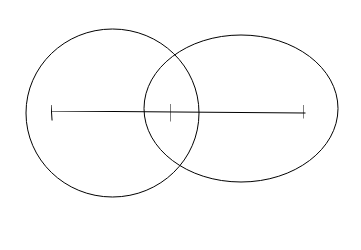
\includegraphics{3.png}
  \end{center}

  Возьмём $U_1$. В нём есть первообразная $F_1$ по предыдущему следствию, т.к. $f\in\O(D)$. Пусть $\Phi(t):=F_1(\g(t))$ на $[t_0,t_1]$. 

  $U_1\cap U_2\neq \emptyset$, в $U_2\q\exists F_2$ - первообразная и $F_2 - F_1 \equiv const$ на $U_1\cap U_2$ по одной из предыдущих теорем. Тогда выберем $F_2$ так, чтобы $F_2 = F_1$ на $U_1\cap U_2$. Пусть $\Phi(t):=F_2(\g(t))$ на $[t_1,t_2]$.

  Продолжаем построение. Получили $\Phi(t)\in C([0,1])$ - первообразную вдоль пути $\g$. 
    \item Теперь докажем единственность.

    Пусть $\Phi_1,\Phi_2$ - первообразные вдоль пути $\g$. Рассмотрим произвольную т. $t_0\in[0,1]$. Тогда по определению $\exists U_\delta(t_0)\colon \Phi_1(t) = F_1(\g(t))$ и $\Phi_2 = F_2(\g(t))$, где $F_1,\q F_2$ - первообразные $f$ в круге $U_\delta(t_0)$. Значит $F_1 - F_2 \equiv const$  в $U_\delta(t_0)$ $\implies \Phi_1 - \Phi_2 \equiv const$ в $U_\delta(t_0)$ для произвольного $t_0\in[0,1]$.

    Т.к. $\Phi_1 - \Phi_2\in C([0,1])$ и $[0,1]$ - компакт, то по конечному количеству накрытий получаем, что $\Phi_1 - \Phi_2\equiv const$ на $[0,1]$. 
  \end{enumerate}
\end{proof}
\subsection{Формула Ньютона-Лейбница для голоморфной функции}
\begin{theorem}
  $f\in\O(D),\q \g\colon [0,1]\to D$ - гладкий путь, $\Phi$  - первообразная вдоль пути $\g$. Тогда
  \[\int_{\g}f(z)\d z = \Phi(1) - \Phi(0)\]
\end{theorem}
\begin{proof}
    \begin{enumerate}
      \item У $f$ есть первообразная $F$ в $D$:
      \[\implies \Phi(t) = F(\g(t)) + c\]
      \[\implies \Phi(t)' = F'(\g(t))\g(t)' = f(\g(t))\g(t)'\]
      Тогда по определению
      \[\int_{\g}f(z)\d z = \int_{0}^{1}f(\g(t))\g(t)'\d t= \int_{0}^{1}\Phi(t)'\d t = \Phi(1) - \Phi(0)\]
      \item В общем случае разобьём $\g=\bigcup \g_k$ таким образом, что каждый $\g_k\colon[t_{k-1},t_k]\to D\colon \g_k([t_{k-1},t_k])\subset U_k\subset D$, где $U_k$ - круг. Значит в каждом $U_k$ есть первообразная. Тогда по аддитивности интеграла:
      \[\int_{\g}f(z)\d z= \Sum{k=1}{n}\int_{\g_k}f(z)\d z=\Sum{k=1}{n} \left(\Phi(t_{k})- \Phi(t_{k-1})\right)= \Phi(1) - \Phi(0)\]
    \end{enumerate}
\end{proof}
\subsection{Теорема о гомотопии (об интегралах вдоль гомотопных путей)}
\begin{theorem}
  $f\in\O(D)$ и $\g_0\sim\g_1$ в $D$. Тогда
  \[\int_{\g_1}f(z)\d z=\int_{\g_2}f(z)\d z\]
\end{theorem}
\begin{proof}
  Построим отображение из определения гомотопности путей $\g\colon[0,1]^2\to D,\q \g(K_{mn})\subset U_{mn}\subset D$, где $K_{mn}$ - это наслаивающиеся друг на друга прямоугольники по обоим направлениям:
  \begin{center}
  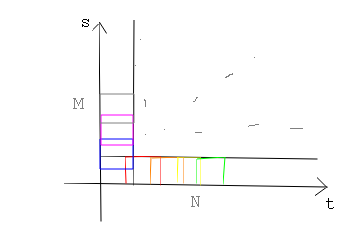
\includegraphics{5.png}
  \end{center}

  $N$ столбцов из прямоугольников по $t$ и $M$ строк из прямоугольников по $s$. Тогда $U_{mn}$ - это наслаивающиеся окружности вокруг образов этих прямоугольников:

  \begin{center}
    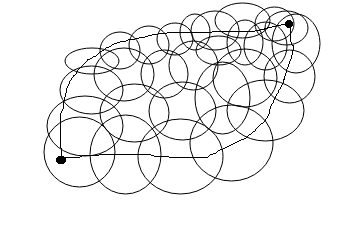
\includegraphics[scale=0.9]{6.png}
  \end{center}

  Важно, чтобы каждый круг пересекался со своими соседями. 

  Пусть $K_m:=\bigcup_{n=1}^NK_{mn}$ и $\Phi_1(s,t) := F_{11}(\g(s,t))$ в $K_{11}$, где $F_{11}$ - первообразная в $\g(K_{11})$. Выберем $F_{12}$ так, чтобы в $\g(K_{11})\cap \g(K_{12})$ $F_{11}=F_{12}$ и пусть $\Phi_1(s,t) := F_{12}(\g(s,t))$ в $K_{12}$; и т.д. ($F_{1,n}=F_{1,n-1}$ в $\g(K_{1,n})\cap \g(K_{1,n-1})$). Получим, что
  \[\forall n\in \left\{1,\dots,N\right\}\q \Phi_1(s,t) = F_{1n}(\g(s,t)) \text{ в $K_{1n}$ }\]
  Значит $\Phi_1\in C(K_1)$. Аналогично строим $\Phi_m\in C(K_m)\q\forall m\in \left\{1,\dots, M\right\}$.

  Рассмотрим теперь $K_{11}$ и $K_{21}$: 
  \[\Phi_1(s,t) = F_{11}(\g(s,t))\]
  \[\Phi_2(s,t) = F_{21}(\g(s,t))\]
  Заметим, что $F_{11} - F_{21}\equiv const$ на $U_{11}\cap U_{21}$, значит $\Phi_1 - \Phi_2$ локально постоянна на каждом $K_{1n}\cap K_{2n}$ и непрерывна на $K_1\cap K_2$, а значит $\Phi_1-\Phi_2 \equiv const$ на $K_1\cap K_2$. Тогда можно выбрать $\Phi_2$ так, чтобы $\Phi_1=\Phi_2$ на $K_1\cap K_2$. Аналогично выбираем $\Phi_n$ так, чтобы $\Phi_n=\Phi_{n-1}$ на $K_n\cap K_{n-1}$. 

  Пусть тогда $\Phi(s,t):=\Phi_m(s,t)$ на $K_m$. Заметим, что $\Phi(s,t)$ - первообразная вдоль пути $\g_s(t)$, значит по теореме Ньютона-Лейбница: 
  \[\forall s\in[0,1]\q \int_{\g_s}f(z)\d z= \Phi(s,1) - \Phi(s,0)\]
  Рассмотрим случаи:
  \begin{enumerate}
    \item Пути $\g_1,\g_0$ не замкнутые. 

    \[\Phi(s,0) = F_{m1}(\g(s,0))=F_{m1}(a)\q s\colon (s,t)\in K_m\]
    где $a:=\g(s,0)\q \forall s\in[0,1]$ по определению. Т.к. $\Phi(s,0)$ получилась локально постоянной ($F_{m1}(a)$ при $s\colon (s,t)\in K_m$) и т.к. $\Phi(s,0)\in C([0,1])$, то $\Phi(s,0)\equiv const$, т.е. не зависит от $s$. Аналогично получаем, что $\Phi(s,1)$ не зависит от $s$, а тогда
    \[\int_{\g_0}f(z)\d z = \Phi(0,1) - \Phi(0,0) = \Phi(1,1) - \Phi(1,0) = \int_{\g_1}f(z)\d z\]

    \item Пути $\g_1,\g_0$ замкнутые. 

    Рассмотрим $\Phi(s,1) - \Phi(s,0) = F_{mN}(\g(s,1)) - F_{m1}(\g(s,0))$, и пусть $a_s := \g(s,1)=\g(s,0)$. Тогда $\Phi(s,1) - \Phi(s,0) \equiv const$ для $s\colon (s,t)\in K_m$, т.е. $\Phi(s,1) - \Phi(s,0)$ локально постоянна и непрерывна на $[0,1]$, а значит $\Phi(s,1) - \Phi(s,0)\equiv const$ на $[0,1]$, а тогда
    \[\oint\limits_{\g_0}f(z)\d z=\Phi(0,1)-\Phi(0,0) = \Phi(1,1) - \Phi(0,0) = \oint\limits_{\g_1}f(z)\d z\]
  \end{enumerate}
\end{proof}
\subsection{Теорема о существовании первообразной в односвязной области}
\begin{theorem}
  $D$ - односвязная область, $f\in\O(D)$. Тогда $\exists F$ - первообразная $f$ в $D$. 
\end{theorem}
\begin{proof}
  Выберем произвольную т. $a\in D$ и рассмотрим
  \[F(z):= \int_{az}f(\zeta)\d \zeta\]
  где $az$ - это любой путь от т. а до т. $z\in D$. Заметим, что $F(z)$ не зависит от выбора пути по ИТК.

  Рассмотрим $h\colon z+h\in D$ и $[z,z+h]\subset D$. Тогда
  \[F(z+h)-F(z) = \int_{[z,z+h]}f(\zeta)\d \zeta\]
  Значит:
  \[\left|\frac{F(z+h)-F(z)}{h}-f(z)\right| = \left|\frac{1}{h} \int_{[z,z+h]}f(\zeta)-f(z)\d \zeta\right|\leqslant \frac{1}{|h|}\cdot |h|\cdot \Sup{[z,z+h]}\left|f(\zeta)-f(z)\right|\underset{h\to0}{\to}0\]
  Значит $F'(z) = f(z)\q\forall z\in D$.
\end{proof}
\subsection{Интегральная формула Коши}
\begin{theorem}
  $f\in\O(G),\q \overline{D}\subset G,\q \partial D$ - простая. Тогда $\forall z\in D$
  \[f(z) = \frac{1}{2\pi i} \oint\limits_{\partial D^+}\frac{f(\zeta)}{\zeta - z}\d \zeta\]
\end{theorem}
\begin{proof}
  Т.к. $D$ открыта, то $\exists U_r = \left\{|\zeta - z|=r\right\}\colon \overline{U_r}\subset D$. Рассмотрим $D_r:=D\setminus U_r$. Применим ИТК для многосвязной области:
  \[0=\oint\limits_{\partial D_r^+}g(\zeta)\d \zeta = \oint\limits_{\partial D^+}g(\zeta)\d \zeta - \oint\limits_{\partial U_r^+}g(\zeta)\d \zeta\]
  где $g(\zeta):=\frac{f(\zeta)}{\zeta-z}\in \O(D_r)$. Значит $\oint\limits_{\partial D^+}g(\zeta)\d \zeta = \oint\limits_{\partial U_r^+}g(\zeta)\d \zeta\implies$ правая часть не зависит от $r$.

  Теперь докажем, что
  \[\oint\limits_{\partial U_r^+}\frac{f(\zeta)}{\zeta-z}\d \zeta=2\pi i f(z)\]

  Знаем, что
  \[\oint\limits_{|\zeta-z|=\e}\frac{1}{\zeta-z}\d \zeta = 2\pi i\implies 2\pi i f(z) = \oint\limits_{|\zeta-z|=\e}\frac{f(z)}{\zeta-z}\d \zeta\]
  Тогда:
  \[\left|\oint\limits_{\partial U_r^+}\frac{f(\zeta)}{\zeta-z}\d \zeta-2\pi i f(z)\right|=\left|\oint\limits_{\partial U_r^+}\frac{f(\zeta) - f(z)}{\zeta-z}\d \zeta\right|\leqslant \oint\limits_{\partial U_r^+}\left|\frac{f(\zeta) - f(z)}{\zeta-z}\right|\d \zeta\leqslant \frac{2\pi i}{r}\cdot \Sup{\zeta \in \partial U_r} |f(\zeta)-f(z)|\underset{r\to0}{\to}0\]
  Но $\oint\limits_{\partial U_r^+}\frac{f(\zeta)}{\zeta-z}\d \zeta$ не зависит от $r$, значит
  \[\oint\limits_{\partial U_r^+}\frac{f(\zeta)}{\zeta-z}\d \zeta=2\pi i f(z)\implies f(z) = \frac{1}{2\pi i}\oint\limits_{\partial U_r^+}\frac{f(\zeta)}{\zeta-z}\d \zeta=\frac{1}{2\pi i}\oint\limits_{\partial D^+}\frac{f(\zeta)}{\zeta-z}\d \zeta\]
\end{proof}
\subsection{Теорема Тейлора для голоморфных функций (о разложимости голоморфной функции в ряд
Тейлора)}
\begin{theorem}
  $f\in\O(D)$ и $U_R(a)\subset D$. Обозначим:
  \[c_n:= \frac{1}{2\pi i} \oint\limits_{|z-a|=r}\frac{f(\zeta)}{(\zeta-a)^{n+1}}\d \zeta\text{, где $0<r<R,\q n\in\N_0$}\]
  Тогда числа $c_n$ не зависят от выбора числа $r$, ряд $\Sum{n=0}{+\infty}c_n(z-a)^n$ сходится в $U_R(a)$, причём к $f(z)$, т.е. $\forall z\in U_R(a)$
  \[f(z) = \Sum{n=0}{+\infty}c_n(z-a)^n\]
  Числа $c_n$ называются коэффициентами Тейлора функции $f$ в точке $a$, а ряд - рядом Тейлора функции $f$ в точке $a$.
\end{theorem}
\begin{proof}
  По ИТК для многосвязной области, $G:=\left\{|z-a|>r_1,\q |z-a|<r_2\right\},\q 0<r_1<r_2<R:$
  \[\oint\limits_{\partial G^+}f(z)\d z=0\]
  т.е.
  \[\oint\limits_{|z-a|=r_2^+}f(z)\d z = \oint\limits_{|z-a|=r_1^+}f(z)\d z\]
  Значит $c_n$ не зависит от $r$.

  Возьмём произвольную $z\in U_R(a)$ и $r\colon |z-a|<r<R$. Тогда по ИФК:
  \[f(z) = \frac{1}{2\pi i} \oint\limits_{|\zeta - a| = r}\frac{f(\zeta)}{\zeta-z}\d \zeta = \frac{1}{2\pi i} \oint\limits_{|\zeta - a| = r}\frac{f(\zeta)}{\zeta-a+a-z}\d \zeta =\]
  \[=\frac{1}{2\pi i} \oint\limits_{|\zeta - a| = r}\frac{f(\zeta)}{\zeta-a}\cdot \frac{1}{1-\frac{z-a}{\zeta-a}}\d \zeta=\]
  Заметим, что $\left|\frac{z-a}{\zeta-a}\right|=\frac{|z-a|}{r} < \frac{r}{r}=1$, а значит это бесконечная геометрическая прогрессия:
  \[=\frac{1}{2\pi i} \oint\limits_{|\zeta - a| = r}\frac{f(\zeta)}{\zeta-a}\cdot \Sum{n=0}{+\infty}\left(\frac{z-a}{\zeta-a}\right)^n\d \zeta = \frac{1}{2\pi i} \oint\limits_{|\zeta - a| = r}\Sum{n=0}{+\infty}\frac{f(\zeta)}{(\zeta-a)^{n+1}}\cdot (z-a)^n\d \zeta\]
  Пусть $M:=\Sup{|\zeta-a|=r}|f(\zeta)|$, тогда
  \[\left|\frac{f(\zeta)}{(\zeta-a)^{n+1}}\cdot (z-a)^n\right|\leqslant \frac{M|z-a|^n}{r^{n+1}}=\frac{M}{r}\cdot \left|\frac{z-a}{r}\right|^n\]
  где $\left|\frac{z-a}{r}\right|<1$. Значит $\Sum{n=0}{+\infty}\frac{M}{r}\left|\frac{z-a}{r}\right|^n$ сходится как сумма геометрической прогрессии, а тогда исходная сходится равномерно на контуре. Теперь можно переставить их местами:
  \[\frac{1}{2\pi i} \oint\limits_{|\zeta - a| = r}\Sum{n=0}{+\infty}\frac{f(\zeta)}{(\zeta-a)^{n+1}}\cdot (z-a)^n\d \zeta=\Sum{n=0}{+\infty}\left((z-a)^n\frac{1}{2\pi i}\oint\limits_{|\zeta - a| = r}\frac{f(\zeta)}{(\zeta-a)^{n+1}}\d \zeta\right)=\]
  \[=\Sum{n=0}{+\infty}(z-a)^nc_n\]
\end{proof}
\subsection{Неравенства Коши для коэффициентов Тейлора}
\begin{theorem}
  В условиях теоремы Тейлора
  \[|c_n|\leqslant \frac{M(r)}{r^n}\text{, где $M(r):=\Sup{|z-a|=r}|f(z)|$}\]
\end{theorem}
\begin{proof}
  \[|c_n|=\left|\frac{1}{2\pi i}\oint\limits_{|\zeta - a| = r}\frac{f(\zeta)}{(\zeta-a)^{n+1}}\d \zeta\right|\leqslant \frac{1}{2\pi}M(r)\cdot \frac{1}{r^{n+1}}2\pi r = \frac{M(r)}{r^n}\]
\end{proof}
\subsection{Теорема Лиувилля}
\begin{theorem}
  $f\in\O(\C)$ и $f\in{\rm B}(\C)$. Тогда $f\equiv const$.
\end{theorem}
\begin{proof}
  Пусть $\forall z\in\C\q|f(z)|\leqslant M$.
  Возьмём $a=0$ и построим ряд Тейлора в т. $a$ бесконечного радиуса. Тогда $\forall r>0\q |c_n|\leqslant \frac{M(r)}{r^n}\leqslant \frac{M}{r^n}\to 0$. Значит $c_n=0\q\forall n\geqslant 1$. Итого: $f(z)=c_0\implies f\equiv const$
\end{proof}
\subsection{Теорема Коши-Адамара}
\begin{theorem}
  Пусть дан степенной ряд $\Sum{n=0}{+\infty}b_n(z-a)^n$, $L:=\uplim{n}{\infty}\sqrt[n]{|b_n|}$. Положим
  \[R:= 
  \begin{cases}
    \infty, &L=0\\
    0, &L=\infty\\
    \frac{1}{L}, &\text{иначе }\\
  \end{cases}\]
  \begin{enumerate}
    \item Если $R=0$, то ряд сходится в $z=a$ и расходится в $\C\setminus \left\{a\right\}$ 
    \item Если $R=\infty$, то ряд сходится в $\forall z\in\C$ 
    \item Если $R\neq 0,\infty$, то ряд сходится в $U_R(a)$ и расходится при $z\colon |z-a|>R$. 
  \end{enumerate}
\end{theorem}
\begin{proof}
  \begin{enumerate}
    \item $z=a$ - сходится.
    \item $z\neq a,\q L=\infty\implies \exists \left\{n_k\right\}\colon \exists K\in \N\colon \forall k > K \q \sqrt[n]{|b_{n_k}|}>\frac{1}{|z-a|}$. Тогда $\sqrt[n]{|b_{n_k}|}|z-a|>1\implies |b_{n_k}||z-a|^n>1\not\to 0\implies$ ряд расходится. 
    \item $z\neq a,\q L=0$. Значит $\sqrt[n]{|b_n|}\to 0\implies \exists N\in\N\colon \forall n>N\q \sqrt[n]{|b_n|}<\frac{1}{2|z-a|}\implies \sqrt[n]{|b_n|}|z-a|<\frac{1}{2}\implies |b_{n_k}||z-a|^n<\frac{1}{2^n}$. Значит ряд сходится абсолютно и равномерно по теореме Вейерштрасса. 
    \item $z\neq a,\q L\neq 0,\q\infty$.
    \begin{enumerate}
      \item $|z-a|<R=\frac{1}{L}\implies \exists \e>0\colon |z-a|<\frac{1}{L+\e}$. Т.к. $L=\uplim{n}{\infty}\sqrt[n]{|b_n|}<\infty$, то $\exists N\in\N\colon \forall n\geqslant N \q\sqrt[n]{|b_n|}<L+\frac{\e}{2}\implies \sqrt[n]{|b_n|}|z-a|<(L+\frac{\e}{2})\cdot \frac{1}{L+\e}<1$. Значит ряд сходится по радикальному признаку Коши.
      \item $|z-a|>R=\frac{1}{L}\implies \exists \e>0\colon |z-a|>\frac{1}{L-\e}$. Т.к. $L=\uplim{n}{\infty}\sqrt[n]{|b_n|}$, то $\exists \left\{n_k\right\}\colon\exists K\in\N\colon \forall k\geqslant K \q\sqrt[n]{|b_{n_k}|}>L-\e\implies \sqrt[n]{|b_{n_k}|}|z-a|>(L-\e)\cdot \frac{1}{L-\e}=1$. Значит 
        $|b_{n_k}||z-a|^n>1\not\to0\implies$ ряд не сходится.  
    \end{enumerate}
  \end{enumerate}
\end{proof}
\subsection{Теорема Абеля (о равномерной сходимости на компакте внутри круга сходимости степенного
ряда)}
\begin{theorem}
  Пусть дан степенной ряд $\Sum{n=0}{+\infty}b_n(z-a)^n$, $R$ - его радиус сходимости. Тогда $\forall K$ - компакта $\subset U_R(a)$ ряд сходится на $K$ равномерно.
\end{theorem}
\begin{proof}
  Заметим, что $\forall r<R\q \Sum{n=0}{+\infty}b_nr^n$ сходится, т.к. это $z=a+r$. Рассмотрим функцию $|z-a|$ - она непрерывна на $K\implies \Sup{z\in K}|z-a|=|z_0-a|<R$, где $z_0\in K$ - точка максимума. Обозначим $r:=|z_0-a|$. Тогда на $K$ 
  \[\left|\Sum{n=0}{+\infty}b_n(z-a)^n\right|\leqslant \Sum{n=0}{+\infty}|b_n(z-a)^n|\leqslant \Sum{n=0}{+\infty}|b_n|r^n\]
  а его радиус сходимости $\frac{1}{R}=\uplim{n}{\infty}\sqrt[n]{|b_n|}\implies \Sum{n=0}{+\infty}b_nr^n$ сходится абсолютно. Тогда по теореме Вейерштрасса $\Sum{n=0}{+\infty}b_n(z-a)^n$ сходится абсолютно и равномерно на $K$. 
\end{proof}
\subsection{Теорема о голоморфности суммы степенного ряда}
\begin{theorem}
  $f(z):=\Sum{n=0}{+\infty}b_n(z-a)^n$, $R$ - радиус сходимости. Тогда $f\in\O(U_R(a))$ и $f'(z)=\Sum{n=1}{+\infty}b_n\cdot n(z-a)^{n-1}$ 
\end{theorem}
\begin{proof}
   $\Sum{n=1}{+\infty}b_n\cdot n(z-a)^{n-1}$ сходится в $U_R(a)$, т.к. \[\frac{1}{\tilde{R}}=\uplim{n}{\infty}\sqrt[n]{(n+1)|b_{n+1}|}=\uplim{n}{\infty}\sqrt[n]{|b_{n}|}=\frac{1}{R}\]

   Пусть $g(z):=\Sum{n=1}{+\infty}b_n\cdot n(z-a)^{n-1}$ в $U_R(a)$. Докажем, что $g\in C(U_R(a))$: возьмём произвольную точку $z_0\in U_R(a)\implies \exists \overline{U_\delta(a)}\subset U_R(a)$. Значит по теореме Абеля $g$ сходится равномерно на компакте $\overline{U_\delta(a)}$. Тогда по теореме о непрерывности ряда из непрерывных функций ряд непрерывен на $\overline{U_\delta(a)}\implies g\in C(z_0)\q\forall z_0\in U_R(a)\implies g\in C(U_R(a))$
 
  Пусть $\Delta\colon \overline{\Delta}\subset U_R(a)$
  \[\oint\limits_{\partial\Delta}g(z)\d z = \oint\limits_{\partial\Delta}\Sum{n=1}{+\infty}b_n\cdot n(z-a)^{n-1}\d z=\]
  Т.к. $\partial\Delta$ компакт, то по теореме Абеля $g$ сходится равномерно, а значит можно поменять их местами: 
  \[=\Sum{n=1}{+\infty}b_n\cdot n\oint\limits_{\partial\Delta}(z-a)^{n-1}\d z=0\]
  по Ньютону-Лейбницу, т.к. $\exists \frac{(z-a)^n}{n}$ - первообразная. Тогда по теореме о существовании первообразной в круге $\exists F\colon F'=g$ на $U_R(a)$, где по определению $F\in\O(U_R(a))$. Заметим, что из доказательства той теоремы мы знаем, что $F(z):=\int_{[a,z]}g(\zeta)\d \zeta$ является одной из первообразных $g$. Тогда, т.к. $[a,z]$ - компакт, то $g$ равномерно сходится на нём, а значит:
    \[F(z)=\int_{[a,z]}\Sum{n=1}{+\infty}b_n\cdot n(z-a)^{n-1}\d \zeta=\Sum{n=1}{+\infty}b_n\cdot n\int_{[a,z]}(z-a)^{n-1}\d \zeta=\]
    \[=\Sum{n=1}{+\infty}b_n\cdot n \left(\frac{(\zeta-a)^n}{n}\right)|_a^z=\Sum{n=1}{+\infty}b_n(z-a)^n=f(z) - c_0\]
    Значит $f\in\O(U_R(a))$ и $f'=g$ на $U_R(a)$. 
\end{proof}
\subsection{Теорема о бесконечной дифференцируемости голоморфной функции и связь коэффициентов
Тейлора и производных голоморфной функции}
\begin{theorem}
  $f\in\O(D)$. Тогда $\forall n\in\N\q f^{(n)}\in \O(D)$, причём если $f(z):=\Sum{n=0}{+\infty}c_n(z-a)^n$, то $f^{(k)}(z)=\Sum{n=k}{+\infty}c_n \frac{n!}{(n-k)!}(z-a)^{n-k}$ 
\end{theorem}
\begin{proof}
  $\forall z_0\in D\q\exists U_R(z_0)\subset D\implies$ там $f$ раскладывается в ряд Тейлора: $f(z)=\Sum{n=0}{+\infty}c_n(z-z_0)^n$. Тогда по предыдущей теореме $f\in D(U_R(z_0))$ и $f'(z)=\Sum{n=1}{\infty}nc_n(z-z_0)^{n-1}$ в $U_R(z_0)$.

  Заметим, что по предыдущей теореме, т.к. $f'$ - сумма степенного ряда, то $f'\in\O(U_R(z_0))$. Продолжаем до бесконечности, получая нужный вид для $f^{(k)}(z)$.
\end{proof}
\textbf{Следствие:} $c_n=\frac{f^{(n)}(a)}{n!}$
\begin{proof}
  По теореме в $U_R(a)$ $f^{(k)}(z)=\Sum{n=k}{+\infty}c_n \frac{n!}{(n-k)!}(z-a)^{n-k}\implies f^{(k)}(a)=c_n \frac{k!}{(k-k)!}=c_nk!$ 
\end{proof}
\subsection{Теорема Мореры}
\begin{theorem}
  Пусть $f$ в $D$ удовлетворяет условию треугольника, т.е. $f\in C(D)$ и $\forall \overline{\Delta}\subset D\q \oint\limits_{\partial \Delta}f(z)\d z=0$. Тогда $f\in\O(D)$. 
\end{theorem}
\begin{proof}
  Рассмотрим произвольную точку $z_0\in D$. Так как $D$ открыта, то $\exists U_R(z_0)\subset D\implies$ в $U_R(z_0)$ выполняется условие треугольника, значит там $\exists F\in\O(U_R(z_0))$ - первообразная $f$. Тогда по теореме о бесконечном дифференцировании голоморфной функции $f\in\O(U_R(z_0))$. Т.о., $f\in\O(U_R(z_0))\q\forall z_0\in D\implies f\in\O(D)$.
\end{proof}
\subsection{Теорема о представлении голоморфной функции в окрестности нуля}
\begin{theorem}
  $f\in\O(U(a))$ и $f(a)=0$. Тогда либо $\exists \delta>0\colon f\equiv 0$ в $U_\delta(a)$, либо $\exists \delta>0\colon f(z)=(z-a)^Ng(z)$, где $g\in\O(U_\delta(a))$ и $g(a)\neq0$. 
\end{theorem}
\begin{proof}
  Рассмотрим коэффициенты Тейлора функции $f$ в точке $a$. Знаем, что $c_0=0$. Рассмотрим два случая:
  \begin{enumerate}
    \item $\exists N$ - номер первого $c_n$, который не 0. Тогда
    \[f(z)=\Sum{n=N}{+\infty}c_n(z-a)^n\]
    Пусть $g(z):=\frac{f(z)}{(z-a)^N}=\Sum{n=0}{+\infty}c_{N+n}(z-a)^n\implies g\in\O(U_\delta(a))$. Таким образом, получили, что
    \[f(z)=(z-a)^Ng(z),\q g(a)=c_N\neq 0\]
    \item Такого номера не нашлось. Значит $f\equiv 0$ на $U_\delta(a)$. 
  \end{enumerate}
\end{proof}
\subsection{Теорема об изолированности нулей голоморфной функции}
\begin{theorem}
  $f\in\O(U(a))$ и $f(a)=0$. Тогда либо $f\equiv 0$ в $U_\delta(a)$, либо $\exists\delta>0\colon f(z)\neq 0$ в $\overset{\circ}{U}_\delta(a)$. 
\end{theorem}
\begin{proof}
  Рассмотрим сразу второй случай, так как первый тривиальный: 
  $f(z)=(z-a)^Ng(z),\q g(a)\neq 0\implies \exists U_\delta(a)$, в которой $g(z)\neq 0$, а $(z-a)^N\neq 0$ в $\overset{\circ}{U}(a)$. Значит $f(z)\neq 0$ в $\overset{\circ}{U}_\delta(a)$. 
\end{proof}
\subsection{Теорема единственности для голоморфных функций}
\begin{theorem}
  $f,g\in\O(D),\q E\subset D$, $E$ - множество с предельной точкой в $D$ и $f = g$ в $E$. Тогда $f=g$ в $D$. 
\end{theorem} 
\begin{proof}
 \begin{enumerate}
   \item Пусть $a\in D$ - предельная точка множества $E$. Тогда в силу непрерывности $f(a)=g(a)$. Рассмотрим $h(z):=f(z)-g(z)\implies h(a)=0$ и $a$ - неизолированный 0 (т.к. $\forall \e>0$ есть 0 в $\overset{\circ}{U}_\e(a)\cap E$) голоморфной функции $h\in\O(D)$. Значит по теореме $\exists \delta>0\colon h\equiv 0$ в $U_\delta(a)$. 
   \item Покажем, что $h\equiv 0$ в $D\colon$ пусть нет, т.е. $\exists b\in D\colon h(b)\neq0$. Т.к. $D$ - область, то $\exists \g$ - путь в $D$, соединяющий точки $a$ и $b$, т.е. $\g(0)=a,\q \g(1)=b$. Рассмотрим $h(\g(t))$, пусть $T:=\Inf{t\in[0,1]} \left\{h(\g(t))\neq0\right\}$. Т.к. $h$ непрерывна в $D$ и $h(b)\neq 0$, то $T<1$. Также $T\geqslant \e$, где $\e$ - пересечение $\g$ и $\partial U_\delta(a)$. Таким образом, $T\in(0,1)$.

   По непрерывности $h(\g(T))=0\implies$ это неизолированный 0 (т.к. $\forall \e>0$ есть 0 в $\left\{\g(t),\q 0<t<T\right\}$). Значит $\exists U_\delta(\g(T))\colon h(z)=0$ - но это противоречит с тем, что $T$ инфинум.
 \end{enumerate}
\end{proof}
